\newpage
\section{Qt, PyQt}
\nocite{pyqt:www}

\begin{center}
	
\includegraphics[scale=0.3]{pictures/qt_logo}
\end{center}

V současné době se vývojem Qt zabývá firma Nokia, která Qt koupila v roce 2008 od norské společnosti Trolltech. Společnost Trolltech započala s vývojem Qt v roce 1999. Qt je poměrně mocný soubor nástrojů pro psaní grafických aplikací v jazyce C++. Není to ale pouze knihovna pro psaní GUI. Qt nabízí také řadu programů, které usnadňují vývojáři práci. Například velmi kvalitní IDE v podobě Qt Creator či Qt Designer pro pohodlnou tvorbu grafického rozhraní pouhým přetahováním widgetů myší. Qt Designer umožňuje pohodlně rozvrhnout a umístit jednotlivé widgety, seskupovat je do layoutů či nastavovat parametry. \\
\indent Existuje také mimo jiné verze pro Python - v současnosti verze PyQt4. PyQt je vyvíjena firmou Riverbank Computing. Z rodiny Qt, resp. PyQt, byla v této práci využita samotná knihovna pro psaní kódu, obzvláště pak její Graphics View Framework, a program QtDesigner.

V této podkapitole se také zmíním o architektuře Model View Controller (MVC) a její implementaci v Qt, kterou jsem použil u Processing Manageru (toolbox pro QGIS Processing Framework), a Graphics View Framework, který jsem využil při práci na vizuální stránce práce. V závěru zmíním projekt VisTrails, který byl inspirací při návrhu grafického znázornění Workflow Builderu. 

Pro bližší informace o Qt (i o PyQt4) a jejich možnostech doporučuji oficiální dokumentaci Qt, která je dostupná online a je na velmi vysoké úrovni \cite{qt:www}.

\begin{figure}[h]
	\centering
	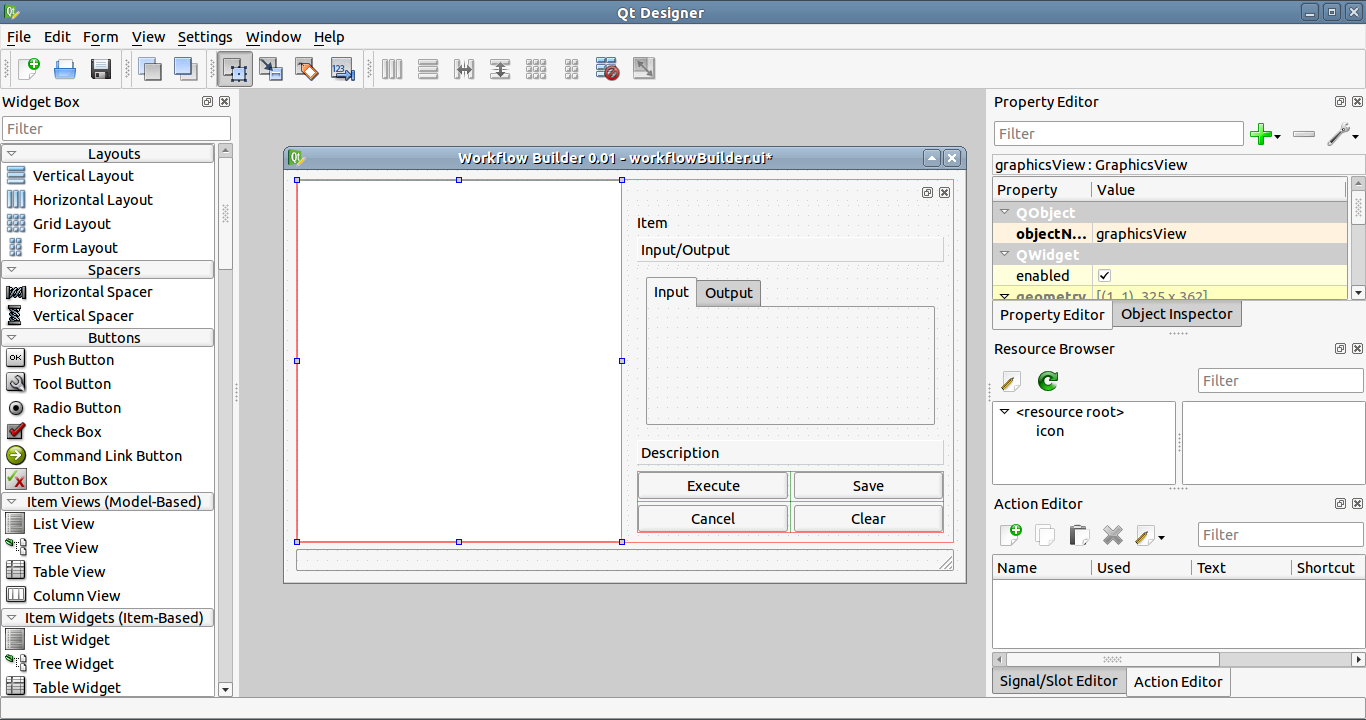
\includegraphics[scale=0.35]{pictures/qt/qt_designer}
	\caption{Qt Designer - nástroj pro tvorbu grafického rozhraní}
  	\label{qtdesigner}
\end{figure}

Soubor vytvořený v Qt Designer (s příponou \textbf{.ui}) lze jednoduše přeložit programem \textbf{pyuic4} do kódu pro Python srozumitelného. \\

\begin{lstlisting}[label=pyuic4,caption={pyuic4 - přeložení .ui souboru do pythoního kódu},morekeywords={pyuic4}]
		pyuic4 soubor_vytvoreny_v_Qt_Designer.ui -o py_soubor.py 
\end{lstlisting}

%%%%%%%%%%%%%%%%%%%%%%%
%%% Signály a sloty %%%
%%%%%%%%%%%%%%%%%%%%%%%
\newpage
\subsection{Signály a sloty}
Každý objekt knihovny Qt, který je potomkem třídy QObject, má své signály a sloty. Signál je to, co objekt vysílá (emituje), má svůj název. Využívá se při různých změnách objektu. Například když klikneme na objekt \textbf{QPushButton}, vyšle se signál \textit{clicked()}. Tento signál poté můžeme zachytit pomocí metody \textit{connect()}, kterou dědí každý takový objekt knihovny Qt od třídy \textbf{QObject}. Takové propojení signálu a slotu může vypadat například takto \textit{connect($kdoVyslal,SIGNAL("clicked()"), SLOT()$)}. Slot je v podstatě metoda či funkce, která se zavolá na základě nějakého podnětu, signálu. 

Signály a sloty v Qt se hojně využívají při tvorbě grafického rozhraní. Jakékoliv kliknutí, změna textu v \textbf{QLineEdit}, změna prvku v \textbf{QComboBox}, změna pozice grafického objektu (\textbf{QGraphicsObject}) či zavření okna vysílají signály. Tyto signály se vysílají bez ohledu, zdali jim nasloucháme či nikoliv. Každá třída má signály a sloty, které dědí po předku, a navíc může obsahovat další, které jsou pro ni typické a mohou se programátorovi hodit. Pakliže nás nějaká změna zajímá, můžeme daný signál zachytit. Kromě toho si můžeme sami napsat svoje vlastní signály či sloty a nemusí se jednat jen o grafické rozhraní. Musíme mít ale na paměti, že objekt, který vysílá signál, musí být potomek objektu \textbf{QObject}. Vyslat signál můžeme  pomocí metody \textit{emit($SIGNAL()$,...)}. V metodě $SIGNAL()$ uvedeme název signálu a dále za ním parametry, které se s ním vyšlou. Signály poté spojíme se slotem pomocí metody $QObject.connect(QObject, SIGNAL, SLOT)$. Tato metoda je statická, tudíž ji můžeme volat přímo z \textbf{QObject}. Slot je metoda, která se spouští na základě signálu.  \\

\noindent Příklad:

Předpokládejme, že $tonda$ je objekt třídy \textbf{Tonda}, která je potomkem třídy \textbf{QObject}. Když jde $tonda$ domů, vyšle signál $SIGNAL("jdu")$ s parametrem $"domu"$: \\


\begin{lstlisting}[label=qtemit,caption={vyslání slotu pod názvem $"jdu"$ s atributem $"domu"$}]
		tonda = Tonda()
		tonda.emit(SIGNAL("jdu"),"domu")
\end{lstlisting}

Marie je také potomek třídy \textbf{QObject} a nachází se kdekoliv. Marie má v sobě zabudovaný slot a jakmile zachytí signál od $tondy$, že odešel, začne jednat: \\


\begin{lstlisting}[label=qtconnect,caption={zachycení signálu $"odesel"$ od tondy}, morekeywords={Marie, SIGNAL, QObject}]
	class Marie(Object):
		def __init__(self):
			QObject.__init__(self)
			self.connect(tonda, SIGNAL("jdu"), self.jednat)
			# mohou nasledovat dalsi spojeni
		
		def jednat(self, parametr):
			# tady se Marie muze rozhodnout na zaklade parametru, 
			# jak bude jednat
			# napriklad:
			if parametr is "domu":
				self.vecere()
		
	marie = Marie()
\end{lstlisting}

\noindent $Tonda$ může emitovat kolik signálů chce a záleží pouze na tom, kolika signálům bude $marie$ naslouchat.

%%%%%%%%%%%%%%%%%%%%%%%%%%%%%%
%%% Model/View Programming %%%
%%%%%%%%%%%%%%%%%%%%%%%%%%%%%%
\subsection{Model-View architektura}
Při seznamování s projektem QGIS Processing Framework a po komunikaci s Camilo Polymeris (student, který začal psát QGIS Processing Framework), jsem začal s přepsáním Processing Manageru (panelu s moduly) z QTreeWidget do MVC architektury. Standardní MVC architektura dělí aplikaci do tří částí, které jsou na sobě co nejméně závislé. Jsou to Model, View a Controller. Oddělení dat od aplikační a prezentační logiky dělá kód přehlednější a lépe udržitelným. Velkou výhodou také je, že jeden model se může zobrazit v několika různých pohledech vždy jiným způsobem.

\begin{figure}[h]
	\centering
	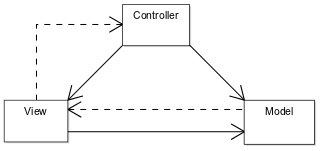
\includegraphics[scale=0.7]{pictures/qt/mvc}
	\caption{Propojení jednotlivých částí architektury MVC}
	\label{mvc}
\end{figure}

\begin{itemize}
	\item{\textbf{Model}} se stará o data - není to pouze místo, kde jsou uložená data, ale jsou zde také definována pravidla, kterýma se jednotlivá data řídí
	\item{\textbf{View}} se stará o zobrazení dat v Modelu a o uživatelské rozhraní
	\item{\textbf{Controller}} spravuje reakce na uživatelovy podněty % má na starosti běh událostí, aktualizaci modelu, aplikační logiku
\end{itemize}

V Qt se implementace MVC architektury objevila s verzí Qt4 v podobě model-view-delegate, kde funkci $controller$u částečně přebírá $view$ (pohled) a částečně $delegate$ (delegát). Delegát určuje, jak budou data editována, případně zobrazena, a komunikuje přímo s pohledem a s modelem. V některých případech může pohled zastávat funkci delegáta. Jedná se o případy, kdy se data editují pomocí jednoduchých editačních nástrojů jako je například editace pomocí \textbf{QLineEdit} u řetězců. Mluvíme tedy o model/view architektuře. Jednoduchý příklad, kde je možné vidět použití hierarchicky uložených dat do modelu a zobrazených ve stromovém pohledu lze najít v \textbf{Příloze A - ukázka použití model/view architektury v PyQt4}. V příkladu uvedeném v téže příloze je také vidět použití vlastního delegáta a proxy modelu pro vyhledávání mezi daty.

\begin{figure}[h]
	\centering
	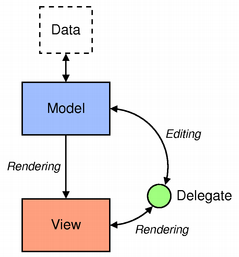
\includegraphics[scale=0.7]{pictures/qt/mv}
	\caption{model-view architektura v Qt4}
	\label{mvc}
\end{figure}

\begin{itemize}
	\item{\textbf{Model}} - tady se nic nemění oproti standardní MVC architektuře; komunikuje se zdrojem dat a poskytuje API pro ostatní komponenty architektury ($view$ a $delegate$)
	\item{\textbf{View}} - zobrazuje data a navíc nabízí základní nástroje pro jejich editaci
	\item{\textbf{Delegate}} - delegát můžeme definovat vlastní widgety sloužící k editaci dat z Modelu; může také definovat, jak se budou jaká data zobrazovat
\end{itemize}

Komunikace mezi jednotlivými komponentami probíhá pomocí signálů a slotů. Qt pro každý prvek architektury ($model$, $view$ a $delegate$) poskytuje základní čistě abstraktní třídy plus několik dalších tříd již přímo použitelných implementací. Například pro data z tabulky můžeme přímo využít \textbf{QTableModel} a \textbf{QTableView}. Pakliže nám žádná z tříd nevyhovuje, můžeme samozřejmě reimplementovat třídy již existující.

\subsubsection*{Model}
Každý model je založený na abstraktní třídě \textbf{QAbstractItemModel}. Pakliže budeme chtít zobrazovat data jako seznam či v tabulce, můžeme se poohlédnout po dalších abstraktních třídách \textbf{QAbstractListModel}, resp. \textbf{QAbstractTableModel} implementující další prvky, které jsou pro daný model typické. Už z názvu je zřejmé, že žádná z těchto tříd nemůže být použita přímo. Mohou nám posloužit k napsání svých vlastních modelů. Také se můžeme pokusit vybrat si z několika základních modelů, které jsou připraveny k přímému použití. Mezi tyto modely patří například \textbf{QStringListModel} pro seznamy řetězců a \textbf{QStandardModel} pro složitější data. Dále existují typy určené pro přístup do databází \textbf{QSqlQueryModel}, \textbf{QSqlTableModel} a \textbf{QSqlRelationalTableModel} či \textbf{QFileSystemModel}, který poskytuje informace o souborech a složkách na vašem lokálním souborovém systému. Máme tedy několik předpřipravených modelů. Nebudou-li nám plně vyhovovat, můžeme si kteroukoliv třídu vybrat a reimplementovat ji.

Dále existují tzv. proxy modely, které stojí mezi view a "standardním" modelem a poskytují podporu pro zpracování dat.  Například \textbf{QSortFilterProxyModel}, který umožňuje uživateli vytvořit pravidla pro řazení a filtraci dat.

View a Delegate získávají a manipulují s daty uloženými v modelech pomocí indexů třídy \textbf{QModuleIndex} a rolí. Index nám udává pozici v modelu pomocí rodiče, řádku a sloupce. V indexu mohou být uložena různá data pomocí různých rolí.

\begin{table}[h]
	\centering
	\begin{tabular}{|c|c|}
		\hline	
		metoda & popis \\
		\hline
		\hline
		child(int row, int column) & vrací potomka na dané pozici QModelIndex \\
		\hline
		data(int role) & vrací data v podobě QVariant \\
		\hline
		model() & vrací model, ve kterém se nachází daný index \\
		\hline
		parent() & vrací rodiče v podobě QModelIndex \\
		\hline
	 	\multirow{2}{*}{row(), column()} & vrací číslo sloupce/řádku daného \\ 
		 & indexu vůči jeho rodiči \\
		\hline
	\end{tabular}
	\caption{některé metody třídy QModelIndex}
	\label{tab:qmodelindex}
\end{table}

\textit{Role} je celé číslo, na základě kterého můžeme zjistit "roli" dat. Existuje několik základních rolí jako $DisplayRole$(0), $ToolTipRole$(3) či $UserRole$(32). Samozřejmě si můžeme v podstatě zvolit jakékoliv celé číslo. Zde se s oblibou využívá $UserRole$, která reprezentuje nejvyšší číslo z předdefinovaných rolí (například $UserRole$ + celé číslo). Z QModelIndex dostaneme data pomocí metody $data(role)$.

\begin{figure}[h]
	\centering
	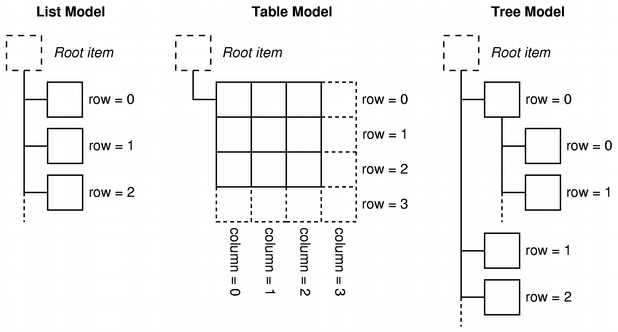
\includegraphics[scale=0.7]{pictures/qt/mv_models}
	\caption{modely v model-view architektuře a jejich pozicování}
	\label{mvModels}
\end{figure} 


Obecně se data do modelu ukládají pomocí metody $setData$(QModelIndex index, QVariant value, int role). Z objektu QVariant můžeme dostat naše data voláním metod jako $toInt()$, $toString()$, $toRect()$... případně $toPyObject()$ [\autoref{qstandarditem}]. 


\begin{table}[h]	
	\centering
	\begin{tabular}{|c|c|}
		\hline	
		metoda & popis \\
		\hline
		\hline
		data(QModelIndex index, int role) & vrací data v podobě QVariant \\
		\hline
		setData(QModelIndex index, QVariant value, int role) & uloží data do modelu \\
		\hline
		insertRow(int row, QModelIndex parent) & vloží data na danou pozici \\
		\hline
		removeRow(int row, QModelIndex parent) & maže data na dané pozice \\
		\hline
		index(int row, int column, QModelIndex parent) & vrací index na dané pozici \\
		\hline


	\end{tabular}
	\caption{některé metody třídy QAbstractItemModel}
	\label{tab:qabsmodel}
\end{table}

U modelu \textbf{QStandardItemModel} se může k položkám v modelu přistupovat také jako \textbf{QStandardItem}. Data se do modelu ukládají jako \textbf{QStandardItem()} objekt. Pro uložení informací do objektu \textbf{QStandardItem} se používá metoda $setData$(QVariant \textit{data}, int \textit{role}). Pakliže nastavíme data pouze pomocí $setData$(\textit{data}), role se nastaví na $UserRole + 1$. Data potom dostaneme z \textbf{QStandardItem} pomocí metody $data(role)$. Model s QStandardItemModel s QStandardItem se hodí pro hierarchicky uspořádaná data. Ukázka použití QStandardItem viz [\autoref{qstandarditem}]. \\

\begin{lstlisting}[label=qstandarditem,caption={QStandardItem - vytvoření a získání dat}, morekeywords={PyQt4, QtCore, QtGui, QStandardItem, Qt, Qt.UserRole, Qt.DisplayRole}]
	from PyQt4.QtCore import Qt
	from PyQt4.QtGui import QStandardItem

	student = QStandardItem("Tonda")
	student.setData(24)
	student.setData("Geoinformatika", Qt.UserRole + 2)

	# vytiskne (24, True) - True znamena, ze se jedna o cislo
	print student.data().toInt() 					
	# vytiskne (24, True)
	print student.data(Qt.UserRole + 1).toInt()		
	# vytiskne "Tonda"
	print student.data(Qt.DisplayRole).toString() 	
	# vytiskne "Geoinformatika"
	print student.data(Qt.UserRole + 2).toString() 	

\end{lstlisting}

Obecně tedy data ukládáme pomocí metody $setData$(data) a získáváme pomocí $data$(), kde na stejnou pozici můžeme uložit více dat s různými rolemi.
 
\subsubsection*{View}

Pomocí pohledů Qt umožňuje zobrazovat data uložená v modelu. Jeden model můžeme zobrazovat v několika různých pohledech. Všechny pohledy jsou potomky abstraktní třídy \textbf{QAbstractItemView}, ta je potomek třídy QAbstractScrollArea a přes QFrame se dostaneme ke třídě \textbf{QWidget}. S pohledy tedy můžeme zacházet jako s ostatními widgety. Model se do view nastaví pomocí metody $setModel$( QAbstractItemModel model). Jednotlivé prvky z modelu jsou pohledu dostupné opět pomocí indexů (QModelIndex). Pohled dokáže prvky zobrazit, řekněme, obyčejně. Pakliže si chceme se zobrazením prvků pohrát více (například měnit font či barvu podle nějakých vlastností dat), použijeme k tomu delegáta. Ten se nastaví pomocí metody $setItemDelegate$(QAbstractItemDelegate delagate). Ukázka nastavení modelu viz [\autoref{qview}]. \\

\begin{lstlisting}[label=qview,caption={View - vytvoření pohledu a nastavení modelu a delegáta}, morekeywords={QItemDelegate, QStandardItemModel, QTreeView}]
	model = QStandardItemModel()
	delegate = QItemDelegate()

	view = QTreeView()
	view.setModel(model)
	view.setItemDelegate(delegate)
\end{lstlisting}

Pro data, která budou zobrazována jako seznam, můžeme využít pohled \textbf{QListView}, pro tabulková data \textbf{QTableView}, pro stromová data pak \textbf{QTreeView}.

\subsubsection*{Delegate}
Všichni delegáti musí být potomky abstraktní třídy \textbf{QAbstractItemDelegate}. Qt nám nabízí k přímému použití třídy QItemDelegate a QStyledItemDelegate. $View$ má defaultně nastaveného delegáta QStyledItemDelegate. Pomocí delegáta můžeme určit, jak se budou dané položky z modelu zobrazovat a jak se budou editovat. 

Pakliže máme v modelu například jako data uloženy studenty a chceme, aby byli vypisováni studenti modře a studentky červeně, můžeme si vytvořit vlastního delegáta, který nám to umožní. V tomto případě [\lstlistingname \ref{qdelegate:paint}] využijeme QItemDelegate a přepíšeme metodu $paint$. \\

\newpage
\begin{lstlisting}[label=qdelegate:paint,caption={Delegate - přepsání metody $paint$}, morekeywords={QItemDelegate, Qt, QFont, AlignLeft, DisplayRole, UserRole, QPen}]
class Delegate(QItemDelegate):
    def __init__(self, parent=None, *args):
        QItemDelegate.__init__(self, parent, *args)

    def paint(self, painter, option, index):
        painter.save()       
        
        # nastaveni fontu
        painter.setPen(QPen(Qt.black))
        painter.setFont(QFont("Times", 10, QFont.Bold))
        
		# nastaveni barvy podle pohlavi
        if index.data(Qt.UserRole + 3).toString() == "female":
            painter.setPen(QPen(Qt.red))
        elif index.data(Qt.UserRole + 3).toString() == "male":
            painter.setPen(QPen(Qt.blue))

        value = index.data(Qt.DisplayRole)
        if value.isValid():
            text = value.toString()
            painter.drawText(option.rect, Qt.AlignLeft, text)
            
        painter.restore()
\end{lstlisting}

        
\noindent V tomto příkladě \ref{qdelegate:paint} předpokládáme, že data (v podobě indexů) obsahují informaci o pohlaví uloženou pod rolí $Qt.UserRole + 3$.

Editor (widget pro editaci dat) nastavíme reimplementací metody $createEditor$, která vrací QWidget. Aby se po editaci změnila data v modelu, musíme také reimplementovat metodu $setModelData$. V [\lstlistingname \ref{qdelegate:createEditor}] předpokládáme, že třída $editStud$ je widget, který je složen ze dvou dalších widgetů - QLineEdit pro editaci jména a QSpinBox pro nastavení věku. \\
\newpage
\begin{lstlisting}[label=qdelegate:createEditor,caption={Delegate - přepsání metod $createEditor$ a $setModelData$}, morekeywords={QItemDelegate, Qt, QFont, AlignLeft, DisplayRole, UserRole, QPen}]
class Delegate(QItemDelegate):
    def __init__(self, parent=None):
        QItemDelegate.__init__(self, parent)
    def createEditor(self, parent, option, index):
    	# editStud je widget slozeny z QLineEdit a QSpinBox
        editor = editStud(index, parent)
        return editor    
    def setModelData(self, editor, model, index):
        model.setData(index,QVariant(editor.name()))
        model.setData(index,QVariant(editor.age()), Qt.UserRole+4)
\end{lstlisting}

Použití QStandardItemModel s QTreeView za použití proxy modelu a delegáta z ukázek \ref{qdelegate:paint} a \ref{qdelegate:createEditor} můžeme dostat výsledek podobný tomuto:

\begin{figure}[h]
	\centering
	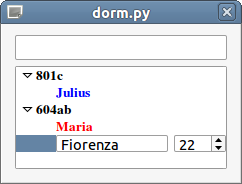
\includegraphics[scale=0.7]{pictures/qt/dorm}
	\caption{Ukázka použití QStandardItemModel, QTreeView, delegáta a proxy modelu.}
	\label{pic:delegate}
\end{figure} 

\noindent
V horní části vidíme widget QLineEdit, který je propojený s proxy modelem a slouží s vyhledávání v datech. Barevně odlišené pohlaví je způsobené delegátem, stejně jako řádek, který se edituje (QLineEdit + QSpinBox). %Celý příklad najdete v příloze.

%%%%%%%%%%%%%%%%%%%%%
%%% Drag and Drop %%%
%%%%%%%%%%%%%%%%%%%%%
\subsection{Drag and Drop}
Zjednodušeně řečeno Drag and Drop je mechanismus, který nám umožňuje vzít jeden objekt z jednoho místa a přesunout ho na místo druhé. A to nejen v rámci jedné aplikace, ale také mezi různými aplikacemi. Na základě 'dopadu' (drop) objektu můžeme vyvolávat různé akce. Můžeme definovat, který objekt může být přetahován nebo které objekty mohou dopadnout na daný objekt (které objekty budou akceptovány). Data se přenáší pomocí objektu \textbf{QDrag}, do kterého se uloží data v podobě \textbf{QMimeData}.

Pro umožnění chytnutí objektu (widgetu) myší přepíšeme metodu $mouseMoveEvent$, která je děděna z \textbf{QWidget}. Zde můžeme nastavit, které tlačítko myši budeme akceptovat a další pravidla na základě kterých se vytvoří či nevytvoří objekt třídy \textbf{QDrag}. 

Akceptování dopadnutých objektů nastavíme metodou $acceptDrops$ s parametrem True. Dále musíme přepsat metodu $dragEnterEvent$(event), $dragMoveEvent$(event) a $dropEvent$(event), kde akceptujeme event (událost) pomocí metody její $accept$(). Jednotlivé události jsou objekty tříd \textbf{QDragEnterEvent}, \textbf{QDragMoveEvent} a \textbf{QDropEvent}. Třída \textbf{QDropEvent} obsahuje metodu $source$(), která nám vrací zdrojový widget \textbf{QDrag} objektu. Pomocí toho se také můžeme rozhodnout, zda danou událost příjmeme či nikoliv.

Tohoto mechanismu jsem využil při přetahování modulů z Processing Manageru do Workflow Builderu. Dále toho také využívá Graphics View Framework při pohybu grafických prvků.

%%%%%%%%%%%%%%%%%%%%%%%%%%%%%%%
%%% Graphics View Framework %%%
%%%%%%%%%%%%%%%%%%%%%%%%%%%%%%%
\subsection{Graphics View Framework}
Graphics View Framework nabízí prostředí pro práci s velkým počtem dvojrozměrných prvků. Nabízí také widget (\textbf{QGraphicsView}), ve kterém se dané prvky zobrazují. Podporuje funkce jako zoom, změna měřítka os nebo rotaci. Prostředí umožňuje spravovat klasické události jako je kliknutí myší, její pohyb či stisknutí klávesy. 

Prostředí staví, podobně jako model-view architektura, na principu, kdy jsou samotná data oddělena od způsobu jejich zobrazení. V Graphics View Framework je model v podobě scény (\textbf{QGraphicsScene}) a pohled zastupuje třída \textbf{QGraphicsView}. Základní třídou dvojrozměrných prvků je \textbf{QGraphicsItem}. Z této třídy se dědí několik dalších jejich reimplementací jako QGraphicsRectItem, QGraphicsPathItem či QGraphicsSimpleTextItem. 

\subsubsection*{QGraphicsItem}
QGraphicsItem je základní třída, ze které vychází ostatní 2D objekty. Pomocí metody $setPos$ se nastaví pozice vůči rodiči. Pakliže žádný rodič není, bere se pozice ve scéně (QGraphicsScene). V Graphics View Framework také funguje hierarchie. Prvkům můžeme nastavit rodiče buď při jejich vytváření, či pomocí metody $setParentItem$(QGraphicsItem parent). Prvkům můžeme nastavit různé vlastnosti jako například jak budou graficky vypadat či zdali mohou být přesouvány. Mezi standardní grafické prvky, které reprezentují klasické tvary, patří:\\
\begin{itemize}
	\item QGraphicsRectItem
	\item QGraphicsPathItem
	\item QGraphicsLineItem
	\item QGraphicsPolygonItem
	\item \ldots
\end{itemize}
 
Prvkům můžeme dále nastavovat tzv. ToolTip pomocí metody $setToolTip$(QString toolTip) či tzv. flagy pomocí $setFlag$(GraphicsItemFlag flag, bool enabled = true) a $setFlags$(GraphicsItemFlags flags). Flagy slouží k nastavení chování prvku. Například chceme-li s prvkem pohybovat, nastavíme flagy QGraphicsItem.ItemIsMovable, QGraphicsItem.ItemIsSelectable a QGraphicsItem.ItemIsFocusable na hodnotu true [viz Ukázka kódu \ref{qgraphicsitem:flags}].\\
 
\begin{lstlisting}[label=qgraphicsitem:flags,caption={Nastavení flagů u QGraphicsRectItem}, morekeywords={QGraphicsItem, QGraphicsRectItem}] 
	rect = QGraphicsRectItem()
	rect.setFlags(QGraphicsItem.ItemIsMovable | \
				  QGraphicsItem.ItemIsSelectable | \
				  QGraphicsItem.ItemIsFocusable)
\end{lstlisting}
 
\subsubsection*{QGraphicsScene}
Obecně se do scény prvky přidávají pomocí metody $addItem$(QGraphicsItem item). U klasických tvarů jako čtyřúhelník, elipsa či linie můžeme použít rovnou metody k tomu určené jako $addRect$(QRectF rect), $addEllipse$(QRectF rect) či $addLine$(QLine line). Prvky se mažou ze scény pomocí $removeItem$(QGraphicsItem item). Pro smazání všech prvků ve scéně slouží metoda $clear$(). Další užitečné metody jsou $items$(), která vrací všechny prvky scény, $itemAt$(QPointF point) vracící prvek na vybrané pozici ve scéně, či $selectedItems$(), která nám vrací seznam prvků, které jsou vybrány.

\subsubsection*{QGraphicsView}
U QGraphicsView nastavíme scénu pomocí $setScene$(). Dále můžeme nastavit možnost přibližování a oddalování, měřítko, barvu pozadí, vyhlazování hran u prvků, můžeme rotovat scénu atp.

Na obrázku Obr. \ref{gsf} je vidět jedna scéna zobrazena ve dvou rozdílných pohledech. Změna scény provedená v jednom pohledu se projeví také v druhém pohledu. U pohledu vpravo byla nastavena barva pozadí pomocí metody $setBackgroundBrush$(QBrush brush), změněno měřítko os pomocí $scale$(int x, int y) a scéna byla otočena o 45$^\circ$ pomocí $rotate$(int angle). \\

\begin{figure}[h]
	\centering
	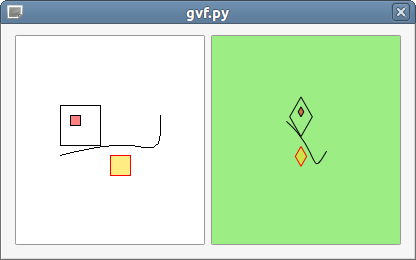
\includegraphics[scale=0.7]{pictures/qt/gsf}
	\caption{Zobrazení jedné scény ve dvou různých pohledech.}
	\label{gsf}
\end{figure}

Při tvorbě vlastního pohledu můžeme reimplementovat metody pro správu Drag and Drop prostředí ($mousePressEvent$, $dragEnterEvent$, $dragMoveEvent$, $dropEvent$...), spravovat vstup z klávesnice ($keyPressEvent$, $keyReleaseEvent$), události vyvolané myší ($mousePressEvent$, $mouseDoubleClickEvent$, $mouseMoveEvent$...) či metodu $wheelEvent$ pro definování chování widgetu při použití prostředního kolečka myši (QWheelEvent je defaultně ignorován).

\subsection{VisTrails}

VisTrails je systém pro správu workflow diagramů vyvíjený na University of Utah. Je napsán v Pythonu za pomoci knihovny PyQt. Systém je open source a uvolněný pod licencí GPL v2. 

Na začátku práce na Workflow Builderu se nabízela možnost využít některých svobodných projektů pro modelování workflow diagramů. Vzhledem k tomu, že QGIS využívá knihovnu Qt a QGIS Processing framework samotný je psaný  v Pythonu, naskýtali se jako možnosti inspirace projekty Orange či \footnotemark{\index{VisTrails} VisTrails}\footnotetext{http://www.vistrails.org/index.php/Main\_Page}.

Nejvíce mě oslovilo grafické zpracování VisTrails [viz Obr. \ref{vt}]. Uživatel na první pohled vidí, jaký parametr je s kterým spojen. Ne pouze který modul je s kterým spojen jak to často bývá u podobných programů. Studoval jsem kód a využil jsem prvky scény \textbf{QGraphicsModule} reprezentující modul, \textbf{QGraphicsPort} reprezentující vstupní a výstupní parametry modulu a \textbf{QGraphicsConnection}, reimplementace třídy QGraphicsPathItem a  reprezentující spojení mezi parametry. Dále jsem se inspiroval postranním panelem, který zobrazuje informace o právě vybraném modulu a umožňuje také nastavování parametrů.

\newpage

\begin{figure}[h]
	\centering
	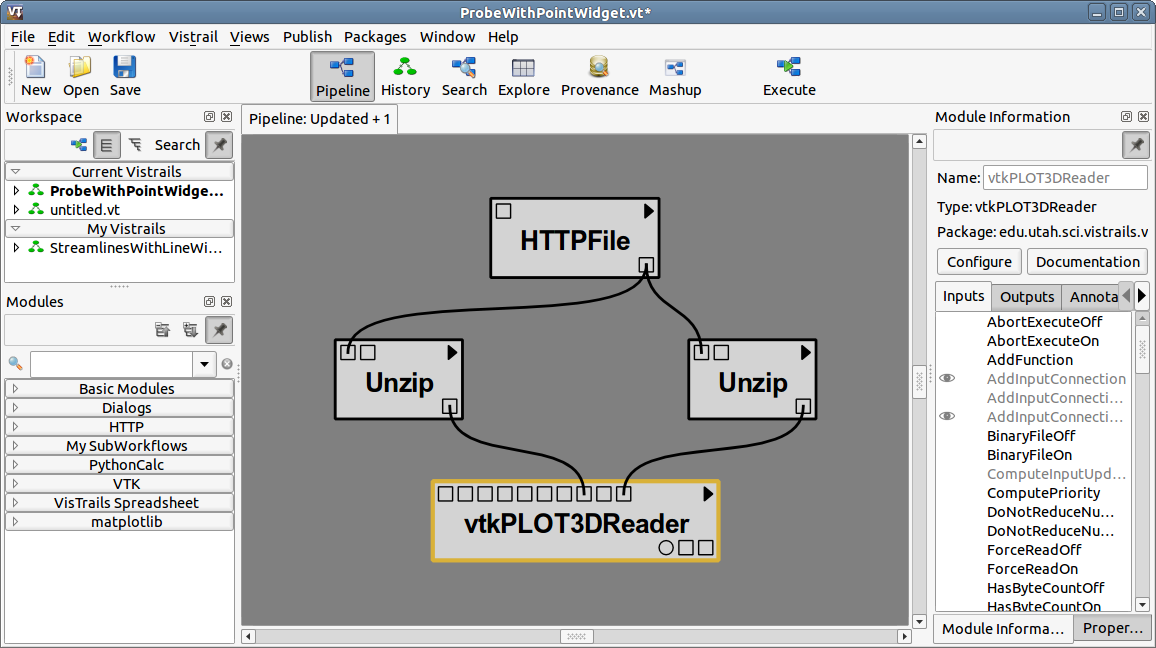
\includegraphics[scale=0.5]{pictures/qt/vt}
	\caption{Ukázka spojení prvků v systému VisTrails.}
	\label{vt}
\end{figure}
